% Generated by thesis/ch7/exp1/bench_figures.py -- do not edit by hand.
\begin{figure}[tbp]
  \centering
  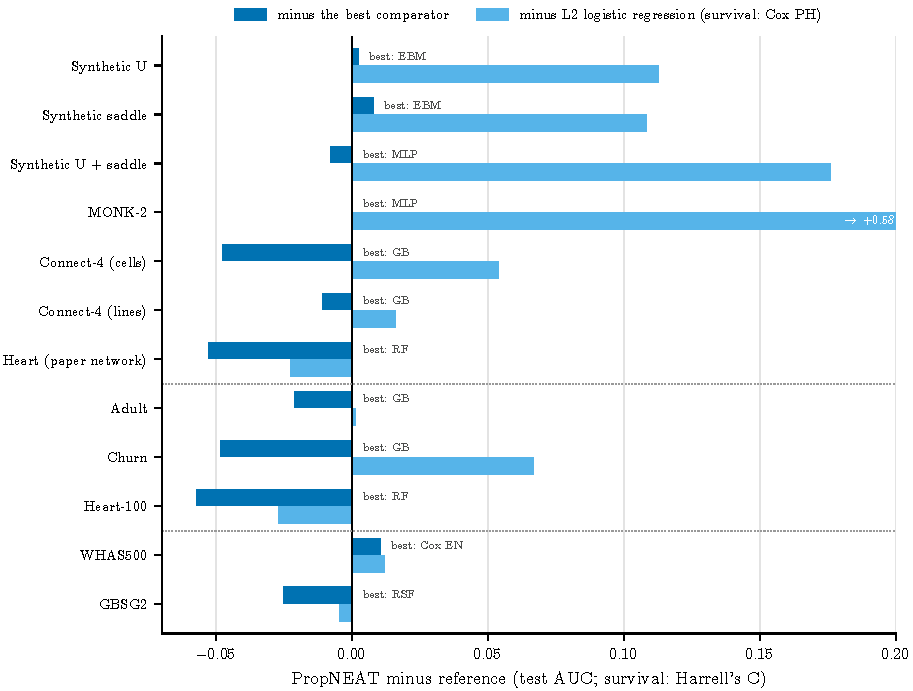
\includegraphics[width=\textwidth,height=0.8\textheight,keepaspectratio]{figures/ch7/options/bench-gap}
  \caption{PropNEAT's test AUC minus the best comparator's and logistic regression's. Dark blue: minus the best comparator (named); light blue: minus logistic regression (survival: Cox PH, Harrell's C); arrow: a bar cut at 0.2, its value printed. LR: logistic regression ($L_2$); L1: $L_1$ logistic regression; RF: random forest; GB: gradient boosting; EBM: explainable boosting machine; MLP: multilayer perceptron; Cox L2 / Cox EN: Cox model with a ridge / elastic-net penalty; RSF: random survival forest; GBS: gradient-boosted survival model.}
  \label{fig:ch7-bench-gap}
\end{figure}
